\subsection{Clocks and reset}
\label{basic:clk_rst}

\begin{figure}[ht]
  \begin{center}
    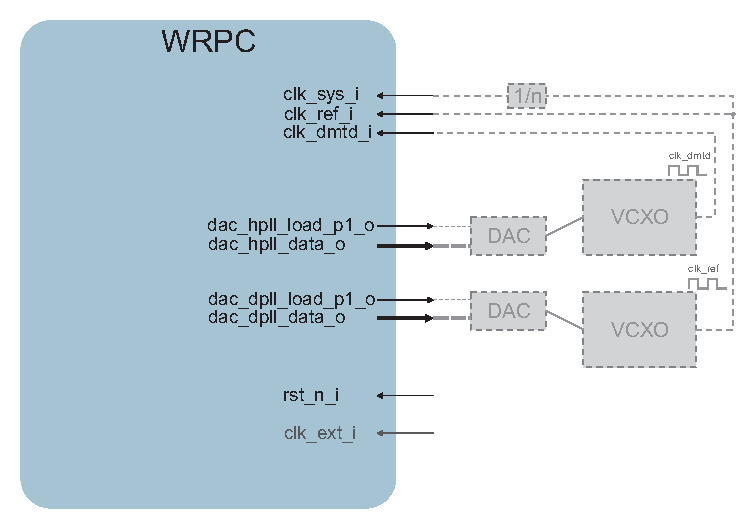
\includegraphics[width=.8\textwidth]{fig/basic_wrpc_clk.pdf}
    \caption{Mandatory clock signals and main reset of WRPC}
  \end{center}
\end{figure}


\begin{center}
  \begin{tabular}{|l|l|p{9cm}|}
    \hline
    %\multicolumn{3}{|l|}{\bf Signals description:}\\
    {\bf Signal name} & {\bf size} & {\bf description} \\
    \hline \hline
    \texttt{clk\_sys\_i} & 1 & main system clock, can be any frequency $\leq
    f_{clk\_ref\_i}$ e.g. 62.5 MHz\\
    \texttt{clk\_dmtd\_i} & 1 & DMTD offset clock (close to 62.5 MHz, e.g. 62.49 MHz)\\
    \texttt{clk\_ref\_i} & 1 & 125 MHz reference clock\\
    \hline
    \texttt{dac\_hpll\_load\_p1\_o} & 1 & validates DAC value on data port \\
    \texttt{dac\_hpll\_data\_o} & 16 & DAC value for tuning helper (DMTD) VCXO\\
    \texttt{dac\_dpll\_load\_p1\_o} & 1 & validates DAC value on data port \\
    \texttt{dac\_dpll\_data\_o} & 16 & DAC value for tuning main (ref) VCXO\\
    \hline
    \texttt{clk\_ext\_i} & 1 & [optional] external 10 MHz reference clock
    input for GrandMaster mode\\
    \texttt{rst\_n\_i} & 1 & main reset input, active-low (hold for at least 5
    \emph{clk\_sys} cycles)\\
    \hline
  \end{tabular}
\end{center}
